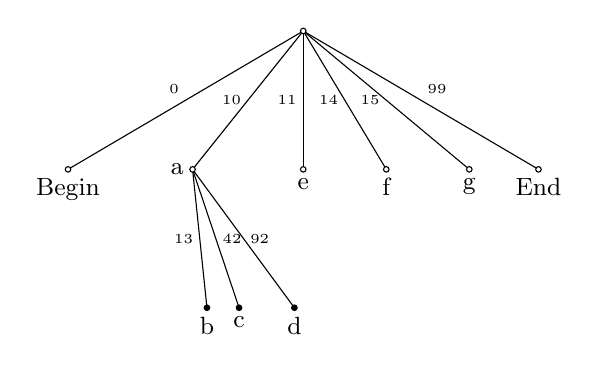
\begin{tikzpicture}[scale=1.0]
\tiny

  
  \draw (0,0) -- node[anchor=south east]{0}  (-85pt, -50pt);
  \draw (0,0) -- node[anchor=south west]{99} ( 85pt, -50pt);

  \draw (0,0) -- node[anchor=east]{10} (-40pt, -50pt);
  \draw (0,0) -- node[anchor=east]{11} (  0pt, -50pt);
  \draw (0,0) -- node[anchor=east]{14} ( 30pt, -50pt);
  \draw (0,0) -- node[anchor=east]{15} ( 60pt, -50pt);

  \draw[fill=white] (0,0) circle (1pt);

\small
  \draw[fill=white] (-85pt, -50pt) node[anchor=north]{Begin} circle (1pt);
  \draw[fill=white] ( 85pt, -50pt) node[anchor=north]{End} circle (1pt);

\tiny
  \draw (-40pt,-50pt) -- node[anchor=east]{13} (-34.8pt, -100pt);
%  \draw (-40pt,-50pt) -- (-30.8pt, -100pt);
  \draw (-40pt,-50pt) -- node[anchor=west]{42} (-23.2pt, -100pt);
%  \draw (-40pt,-50pt) -- (-12.0pt, -100pt);
  \draw (-40pt,-50pt) -- node[anchor=west]{92}(- 3.2pt, -100pt);

\small
  \draw[fill=white] (-40pt, -50pt) node[anchor= east]{\TODO{a}} circle (1pt);
  \draw[fill=white] (  0pt, -50pt) node[anchor= north]{\TODO{e}} circle (1pt);
  \draw[fill=white] ( 30pt, -50pt) node[anchor= north]{\TODO{f}} circle (1pt);
  \draw[fill=white] ( 60pt, -50pt) node[anchor= north]{\TODO{g}} circle (1pt);

  \filldraw[black](-34.8pt, -100pt) node[anchor= north]{\TODO{b}} circle (1pt);
%  \filldraw[black] (-30.8pt, -100pt) node[anchor=north]{23} circle (1pt);
  \filldraw[black](-23.2pt, -100pt) node[anchor= north]{\TODO{c}} circle (1pt);
%  \filldraw[black] (-12.0pt, -100pt) node[anchor=north]{70} circle (1pt);
  \filldraw[black](- 3.2pt, -100pt) node[anchor= north]{\TODO{d}} circle (1pt);

\end{tikzpicture}
